\documentclass[11pt,a4paper,twoside]{article}
\usepackage{package/lmuthesis}

\prof{Prof.\ Dr.\ Heinrich Hu{\ss}mann}
\title{}
\author{Changkun Ou}
\email{hi@changkun.us}
\bearbeitungszeitraum{1.7.2018 bis 31.1.2019}
\betreuer{Malin Eiband and Dr. Daniel Buschek}
% \aufgabenstellung{
%     \begin{description}
%         \item[Problem Statement] Under standing user behavior helps designer optimize 
%         their product user experiences. At the same time, user benefits more productive 
%         from it. Since user intents are elusive, changeable and sometimes even undetermined, 
%         predict their behavior usually difficult and impoissible. In most cases, a user may 
%         performs a series of wasted actions before reach an intent destination. 
%         Nevertheless, user intents becomes clear step by step after performs a series of 
%         actions in a given context. 
%         \item[Scope of the Thesis] To tackle the aforementioned challenges, the objective of this thesis is to develop a system that tracking user actions within a website, 
%         As a first step, literature review ...
%         Based on the literature review, a intent model should be developed ...
%         Then a system should implements the ...
%         Nevertheless, user intents becomes clear step by step after performs a series of actions in a given context. 
%         \item[Tasks] conduct a literature review to identify (research) question that simulates user input and predicts user ...
%         \item[Requirements] asdfasdf
%         \item[Keywords] asdfasdf
%     \end{description}
% }
\acknoledgement{
    Thansk to everyone.
}
\abstract{
    Clickstream research emerges since the end of last century and has proliferated in the heart of our Internet world. 
    Trades, public opinions, and almost every traces are precisely recorded on server side log files. 
    The fundamental interaction between client and server stands immutably, 
    despite the fact that mobile devices have governed our daily life.
    In this thesis, we first established a lab study and collected clickstream data of individuals with manually designed nine different web browsing task for three mainstream websites. 
    Each website has three types of tasks, including goal-oriented, fuzzy and exploring browsing task.
    A collected clickstream of a subject is consists of a timestamp based URL and the time duration of a single URL.
    Based on the type of data, we proposed a generic modern clickstream model to characterize client-side user behavior.
    By analyzing the subject traces from our lab study, we seek to archive these goals:
    1) Understanding: to extract the common patterns between subjects and optimize the visiting clickstream pattern for a new user.
    2) Prediction: with given client clickstream, present the future click path more than one step.
    3) Classification: to separate and report whether a user is exploring on the web.
    To archive these goals, we developed a browser plugin as a possible application that predicts the future possible
    click under a visiting session and provides a score that indicates the probability of exploring.
    Furthermore, we generalize the design of our model and plugin communication protocol and
    discussed the possibility of formalizing them as standard Web APIs.
    To the best of our knowledge, this is the first client-side user clickstream study.
}

\begin{document}

\makecover
% \makeaufgabenstellung
% \makededication
\makeabstract
\maketoc


\section{Introduction}
\label{ch:intro}

\subsection{A Brief History of Clickstream Research}

% 起源

The word ``clickstream'' \cite{friedman1995} was first coined in 1995, a media comments 
article introduced a novel concept of tracing cyberlife of users over the nowadays 
``Internet''. Informally, a ``clickstream'' contains a sequence of hyperlinks clicked by a 
website user over time. At the same year, the most popular server software 
Apache HTTP \cite{apache1995http} proxy on the Web was developed with a feature that 
records access log of entries. Afterwards, people realized the potential danger and value 
of tracing cyberspace, which a large discussion of clickstream influences, such as 
frequency based mining of clickstream \cite{brodwin1995}, privacy concerns 
\cite{reidenberg1996governing}, and database schema of session based time series data 
\cite{courtheoux2000database}.

% 搜集 clickstream 带来的推动

Privacy discussion concludes collecting traces over net clearly offence the rights of users,
the practice violates the openness and transparency of a service to a user.
Serious criticism arise the tracing becomes a loss of democratic governance \cite{gindin1997lost}.

Technologies is not guilty. After years of discussion, positive opinion proposes the rules 
\cite{reidenberg1996governing} and regulations \cite{skok1999establishing} in cyberspace,
means of protecting information privacy in cyberspace transactions \cite{kang1997information},
and approaches to resolve conflicting international data privacy \cite{reidenberg1999resolving}.

Meanwhile, bussiness man agilely responses to the concept and immediately initate 
commercial tracking of their customer to improving marketing affects \cite{novick1995}, 
customer service and precise advertisment\cite{reagle1999platform, bucklin2000sticky}, 
even measuring product success \cite{schonberg2000measuring}.

At the turn of this century, common reviews start accept the technology of clickstream,
clickstream data has confirmed by industrial practice, which opens a new era in 
customer service \cite{walsh2000internet}, most of website users start accept their click path data 
be aggregate analysed on the server side \cite{carr2000hypermediation}.

Clickstream data grows fast and becomes plentiful, researchers start convey the original concept of clickstream,
tracking customer selections, into various applications, such as usability testing \cite{Waterson:2002:LOW:506443.506602},
understanding social network sentiment \cite{Schneider:2009:UOS:1644893.1644899}, and developed visualizing
technique to better interpret clickstream data \cite{Waterson:2002:DTU:1556262.1556276}.

Analysis, reports and characterizing of clickstream gains its popularity, Mobasher et al. \cite{Mobasher:2001:EPB:502932.502935}
suggests personalize user based on association rule from their web usage data. Chatterjee et al. \cite{chatterjee2003modeling} 
first proposed E-commerce websites should use clickstream to tracking customer navigation pattern instead of essential choice, 
associating and binding products for observing responses of a customer.

With the arise of characterizing and behavior understanding on clickstream data, more 
and more research proposes methods for the understanding of given server clickstream data.
Padmanabhan et al. \cite{Padmanabhan:2001:PID:502512.502535}
proposed an algorithm to address personalization from incomplete clickstream data, which implies
a security problem potential information leak from clickstream data. 
Moreover, affected by search engine indexing, Lourenco at al. \cite{Lourenco:2006:CWC:1145581.1145634} recommends an approach for
the detection and containment of web crawler based on server side recorded visiting log file.

After a short review of clickstream history, almost all research putforwards their 
methodology based on server recorded clickstream data.
Note that a daily user is always allowed accesses parallel pages and windows simultaneously,
even allow switching across multiple websites for a browsing purpose.
An obvious missing aspect of those papers is the server recorded data tend to incomplete for 
characterizing a visited user, and the log data can only applied on a specific website. 
As an observation, our research no longer surves server side clickstream, 
but focus and contributes to a client side collected clickstream data 
for a real visiting session of a user in a browser.

\subsection{This Thesis}

% 大体上介绍本论文想要研究 clickstream 的内容,
% 这包括如何开展 clickstream 数据的搜集工作,搜集任务是什么,主要使用的方法,
% 以及得出的结论。根据这些结论,文章提出了一个客户端的插件,
% 能够在现代浏览器上支持这样的预测,
% 同时还进一步探讨了此项功能作为浏览器内建功能甚至浏览器 API 的可能性。

% 本文将视线移出服务端点击流数据,将焦点转移到客户端点击流数据,尝试对客户端独立用户的点击流进行解释。
% 本thesis 由以下几个部分组成。

The main part of the thesis is structured in different chapters, and answers the following
three research question groups:

\begin{enumerate}
    \item \textbf{Understanding}: Why collecting clickstream on client-side differs 
        from server-side collecting?
        What are the most significant, identifiable user behaviors and activity patterns 
        can be observed or algorithmically detected in the context of web browsing that 
        indicates information needs,
        and in which form of quantitative data can characterize a definitive boundary to 
        distinguish browsing behaviors of a user?
    \item \textbf{Classification}: How accurate or how affirmative we can model or identify 
        the proposed browsing behaviors progressively that makes an intelligent system 
        serves proactively?
    \item \textbf{Prediction}: How much future movements of a user can be accurately inferred 
        from the context of web browsing, and how much context is required for the prediction?

\end{enumerate}

% 第二章讨论了目前已有的客户端点击流研究。
Chapter \ref{ch:relate} discusses the exitsting user behavior research based on clickstream data firstly. 
Then discussed the evolution of theory regarding information seeking behavior as our experiment foundation.
In addition, we summaried the reason of recent raise of neural approach in different scientific 
area and the state-of-the-art approaches for generic sequence learning, whose proposed in neural network research.
% 第三章介绍了我们的数据类型、模型的设计。
Chapter \ref{ch:model} defined the completion effeciency of a clickstream first, then we
formalizes our proposed sequence to sequence encoder/decoder model for client-side
clickstream as well as the training techniques for the proposed model.
% 第四章详细描述了实验的设计,介绍了每个所设计任务的原因和考虑,讨论了每个所设计的任务中潜在的数据的搜集和分析工作。
In subsequent chapter, Chapter \ref{ch:exp}, we present our experiment for a lab study,
and construe the design reason of context given web browsing tasks for our subjects based on information behavior theory.
% 第五章分析了第四章描述中搜集到的数据,基于 SVM、t-SNE 分析了除了点击流之外的几个特征,定量分析,得出了结论。。。。
% 然后基于第三章中提出的模型,分析了。。。。的结果,得出了。。。的结论。
Afterwards, in Chapter \ref{ch:eval}, based on SVM, t-SNE and our proposed model, 
we conducte a quantitative analysis with described data from our lab study, 
the evaluation shows a very promising results.
% 最后对用户在任务下的点击流进行了可视化,定性分析,进一步讨论了用户的行为,从而进一步验证了我们的结论。。。
Moreover, we visualize the clickstream through directed graph, by combining our traning model outputs,
we also performs a qualitative analysis to all clickstreams, and the analysis gives evidences that further 
verified the correctness of our model.
% 第六章首先介绍了浏览器插件的工作原理,讨论了我们插件的工作架构。介绍了插件的客户端和服务端的实现方案。
In Chapter \ref{ch:app}, as a consequence of our analysis, we developed a browser plugin 
for Google Chrome as a possible application to our model. The plugin can fairly predict 
the next possible visiting pages of a user. In addition, we generalize the design of
our plugin architecture between client and server,
and then discusse the possibilities of being a standard web API to web developers.

% 第七章对整个 thesis 进行了总结,讨论了本文工作中存在的不足以及未来可改进的方向。
In the last two chapters, we discusse the limitations of this work, summarize the findings of our thesis, 
as well as the possible future improvements and directions of the thesis in the final chapter.
\cleardoublepage
\section{Related Works}
\label{ch:relate}
\epigraph{If I have seen further it is by standing on the shoulders of Giants.}{Isaac Newton}

% - 讨论 client-side 的 clickstream 为什么值得研究,比较服务端搜集的 clickstream 产生的明显变化是什么。
% - 讨论现有的 client-side clickstream 研究分别是针对什么方向的,他们的结论主要是什么,都有什么样的改进空间。
% - 以前的 clickstream 只有类别级的分配模型,通过人工设计某个特定网站的马尔科夫模型来学习用户在不同类别之间的跳转概率。但当变为客户端后,数据变得更加充分,用户在一段时间内可能不局限于某个特定的网站,同时可能被其他网站干扰。

In this chapter, we discuss the former research that releats to our work, including
the existing approaches to clickstream behavior modeling, the evolution of information 
behavior theory regarding how it adapts to our digital world, as well as the 
most related recent advances regarding sequence learning.

\subsection{Clickstream Behavior Modeling}

Clickstream behavior research can be traced back to the year when the word ``clickstream''
was invented. Eearly clickstream behavior research studied the navigational behavior
of user \cite{mandese1995clickstreams, brodwin1995} and 
they binary classified clickstream based on the degree of linearity.

Mobasher et al. discovered the effective and scalable techniques \cite{Mobasher:2001:EPB:502932.502935} for Web personalization
by using association rules and built a recommondation system. Goldfrab invistigates \cite{goldfarb2002analyzing} 
the website choice behavior based on clickstream data and suggests that clickstream simulate company strategy changes.
Afterwards, 
Chatterjee et al. \cite{chatterjee2003modeling} first conduct 
the previous research regarding clickstream to an actual commercial website.
They found that clickstream represents an implication that dynamic advertising
based on customer clickstream history influence the future clickstream of the customer
and increase the interaction with the dynamic advertisement.
More techniquely, Ting et al. uses common sequences to find unexpected browsing behavior \cite{Ting:2005:UMF:1092358.1092469},
and then use their findings to improve website design. 

The most recent research evolved the approach of clickstream modeling,
Wang et al.\cite{Wang:2016:UCC:2858036.2858107} proposed a unsupervised appraoch to model clickstream without labeling.
Chi et al. proposed an analysis framework \cite{chi2017towards} for the general understanding of online information behavior
in a specific page. However, their framework only fits for server side collected clickstream other than a real user clickstream.
Then, Wang et al. \cite{Wang:2017:CUB:3127338.3068332} improved their unsupervised appraoch,
and summarized more approaches for clickstream behavior modeling that identifies span ad abuse
for a specific website. Park et al. models and detects a behavior change among student while learning 
based on Poisson process \cite{Park:2017:DCS:3027385.3027430} to
help improve online learning experience. Amo et al. \cite{amo2018learning} further visualizes search-stream
behavior based on student clickstream on a class, and Shimada et al. proves \cite{Shimada:2018:OCD:3170358.3170412}
online change detection while monitoring on student behavior is possible based on a sliding window.

Zaloudek gives an review on the comparasion \cite{mastersthesis} traditional method to model clickstream data,
then proposed a principle component analysis based method for a semi-supervised learning
of clickstream data, however their approach does not work well on clustering task, and 
the best performance is obtained by traditional multilayer perceptron algorithm.
Chandramohan and Ravindran then further investigate the neural approach on clicksteam mining \cite{N:2018:NAB:3152494.3152505},
they verified that complexy LSTM with Attention mechanism is able to capture whether a user
is intent to buy a product or not based on server side collected clickstream.
Surprisingly, Gundala and Spezzano \cite{Gundala:2018:RDH:3184558.3191644} simply use a Lasso
regression based on sofisticated feature engineering 
archived AOC score 0.769 for reader demand hyperlink prediction on Wikipedia clickstream dataset.

Kammenhuber et al. is the first study regarding client side clickstream \cite{Kammenhuber:2006:WSC:1177080.1177110}.
They proposed a finite-state Markov model that models user's search behavior on a level of
topic categories. Unfortunately their dataset are collected from network package traffic,
and did not consider the time a user spend in each page.


% 关于 assistent 的研究
% @article{lieberman1995letizia,
%   title={Letizia: An agent that assists web browsing},
%   author={Lieberman, Henry and others},
%   journal={IJCAI (1)},
%   volume={1995},
%   pages={924--929},
%   year={1995}
% }

\begin{figure}[H]
    \centering
    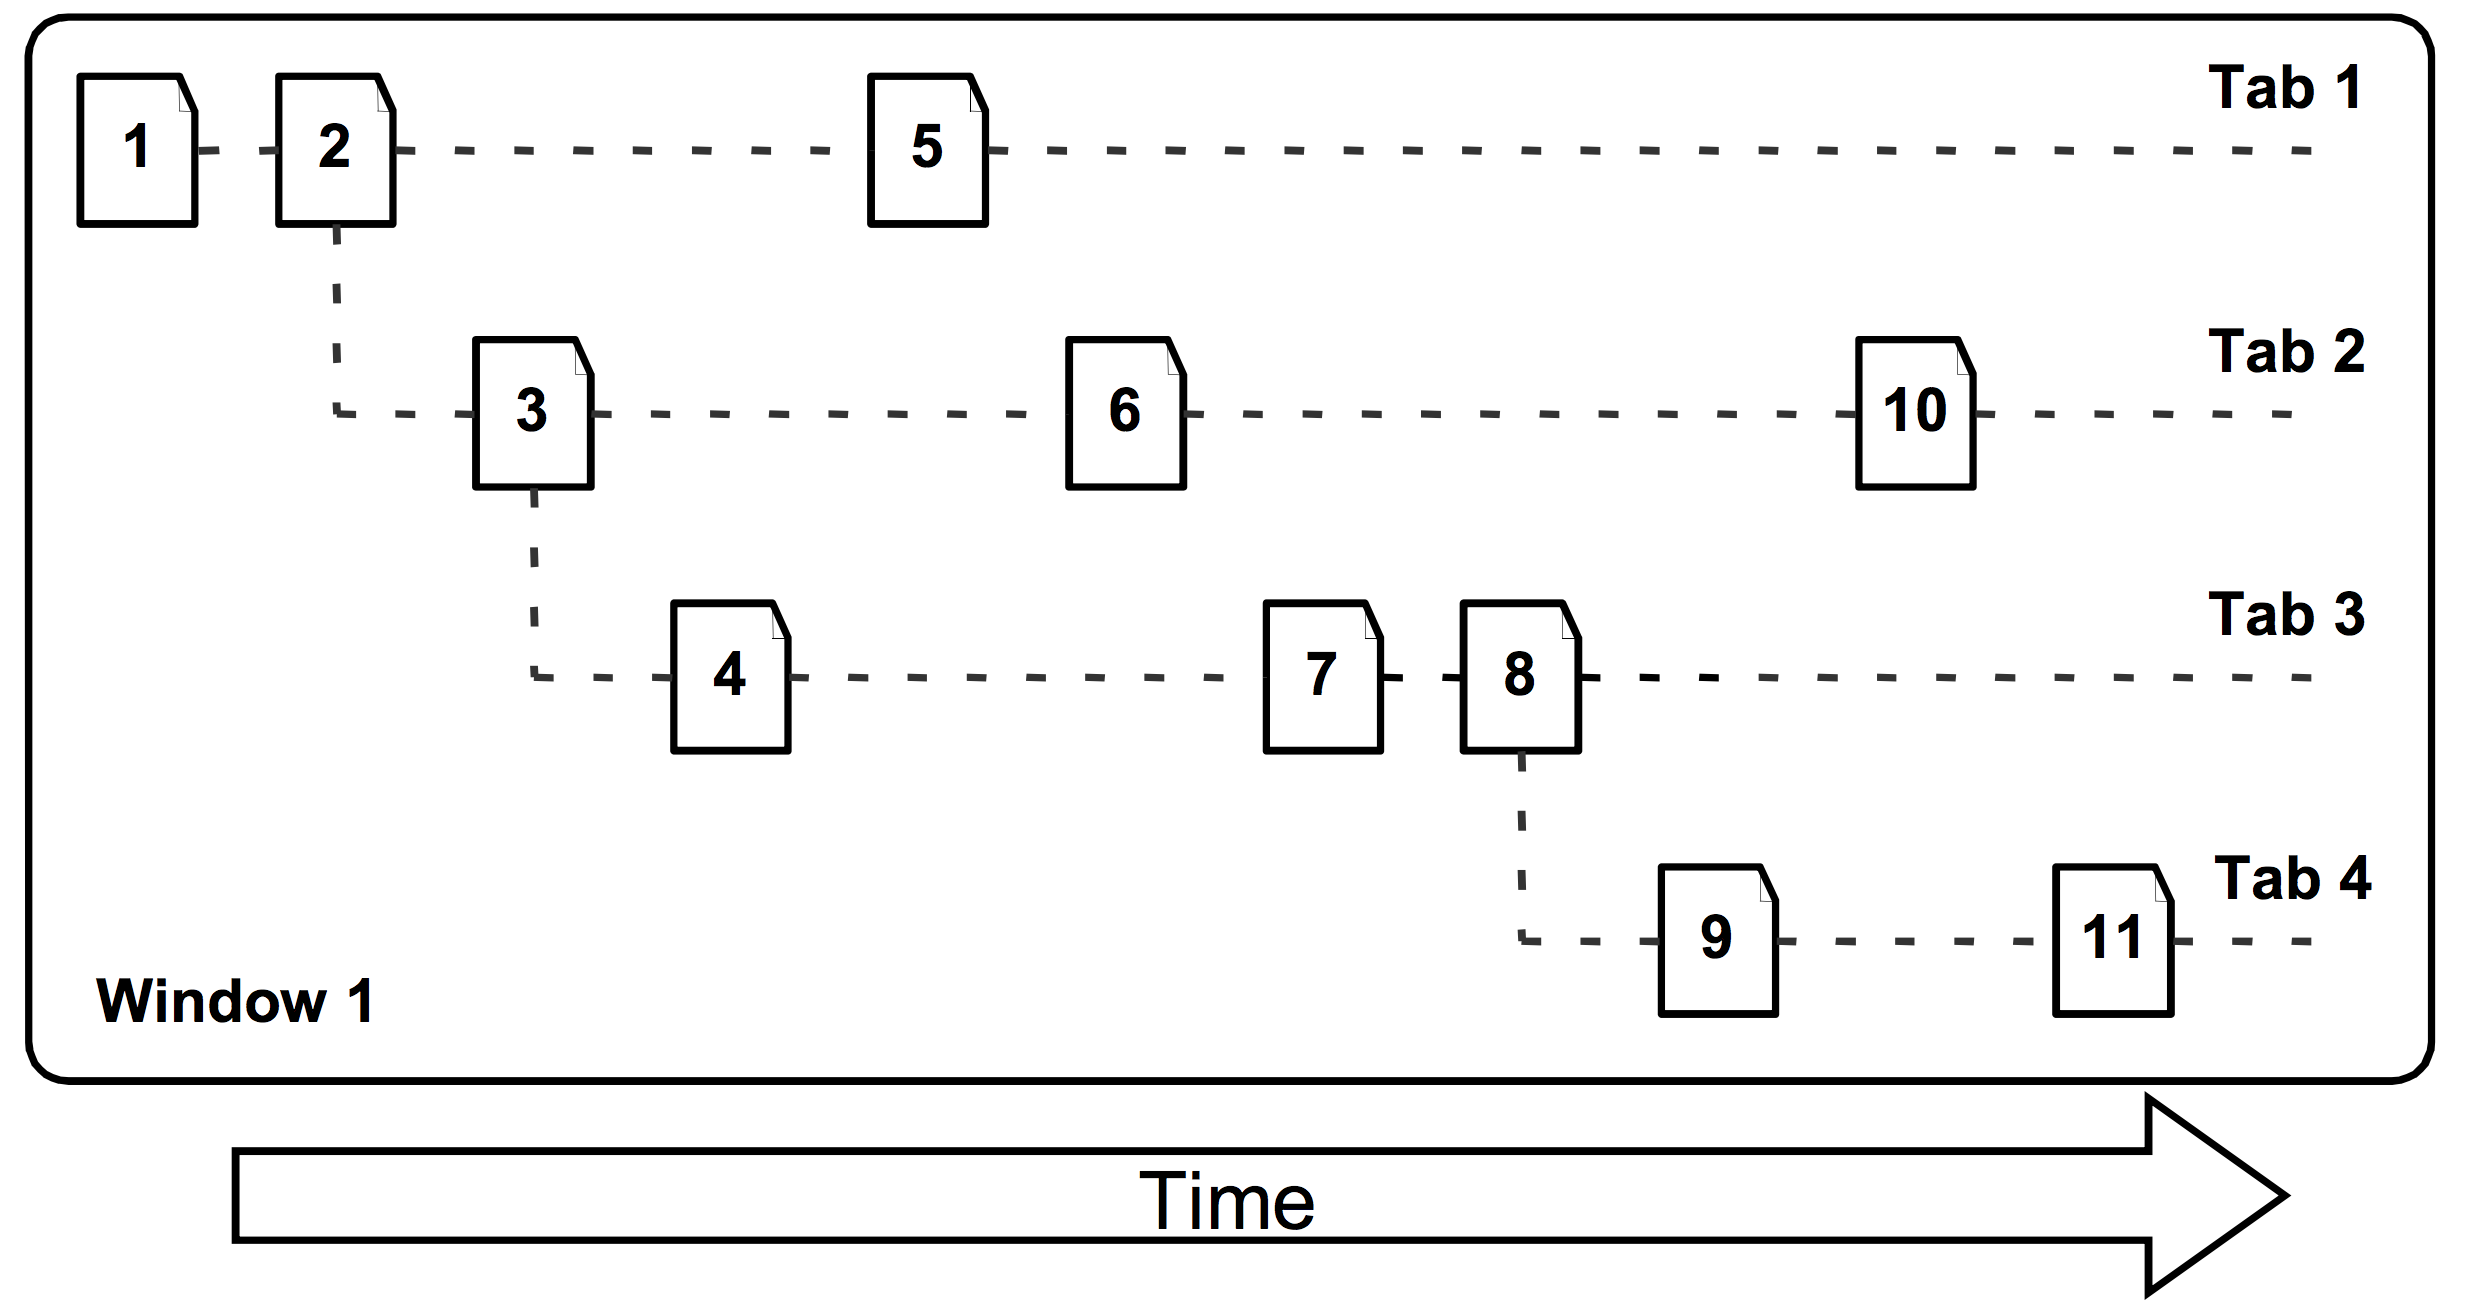
\includegraphics[width=0.55\textwidth]{figures/branching-and-backtracking}
    \caption{Parallel browsing behavior: branching phenomenon \cite{huang2010parallel}}
    \label{fig:backtrace}
\end{figure}

Liu et al. \cite{liu2010understanding} studied a specific user behavior on dwell time on web pages, and concluded that
Weibull distribution is the most appropriate distribution to characterize this behavior. 
Huang et al. \cite{huang2010parallel, huang2012no} further 
noticed the behavior of branching parallel browssing and backtracking browsing
behavior on modern browsers, as shown in Figure \ref{fig:backtrace}, 
and presented an frequent analysis for the distribution of these two behavior individually.

Unfortunately, as we discussed above, the existed research regarding clickstream 
behavior modeling are either server-side modeling for an individual client or 
individually modelized for client-side behaviors with limited information of clickstream,
which does not stands for a real user behavior. 
Besides, the existed approaches are based on self-constructed features, 
the property of Markov memoryless and etc. Though the most recent
approach use neural networks, their findings only applies to specific context.

From the point of view of user behavior, they 
neither unambiguously justifies the foundation of their model, 
nor providing a significative performance of their model.

We, in this thesis, serialize the client side chronologic URL sequences with combines all 
these individually studied phenomena including the branching and backtracking browser 
feature. With this chronologic URLs, we seek to model and understand the essential user 
behaviors patterns while browsing on the Web.

\subsection{Theory of Information Behavior on the Web}
\label{sec:info-seek}

The thesis relates to information behavior theory since it supports the foundation of our
user study. This subsection discusses how the theory was concluded and 
the principles of the theory that sustain our thesis.

Information behavior research encompasses intentional information seeking and 
unintentional information encounters, and the roots to information behavior 
theory relates to information needs and uses \cite{doi:10.1002/aris.2009.1440430114} 
that arose in the 1960s.

However, the concept of information seeking behavior, was coined in late 1981 
by Thomas Wilson \cite{wilson1981user}, and he tries to formalize the process or 
activities of a conscious effort while information needs 
and uses. Figure \ref{fig:wilson-info-seek} illustrate the model of information behavior 
was proposed.

\begin{figure}[H]
    \centering
    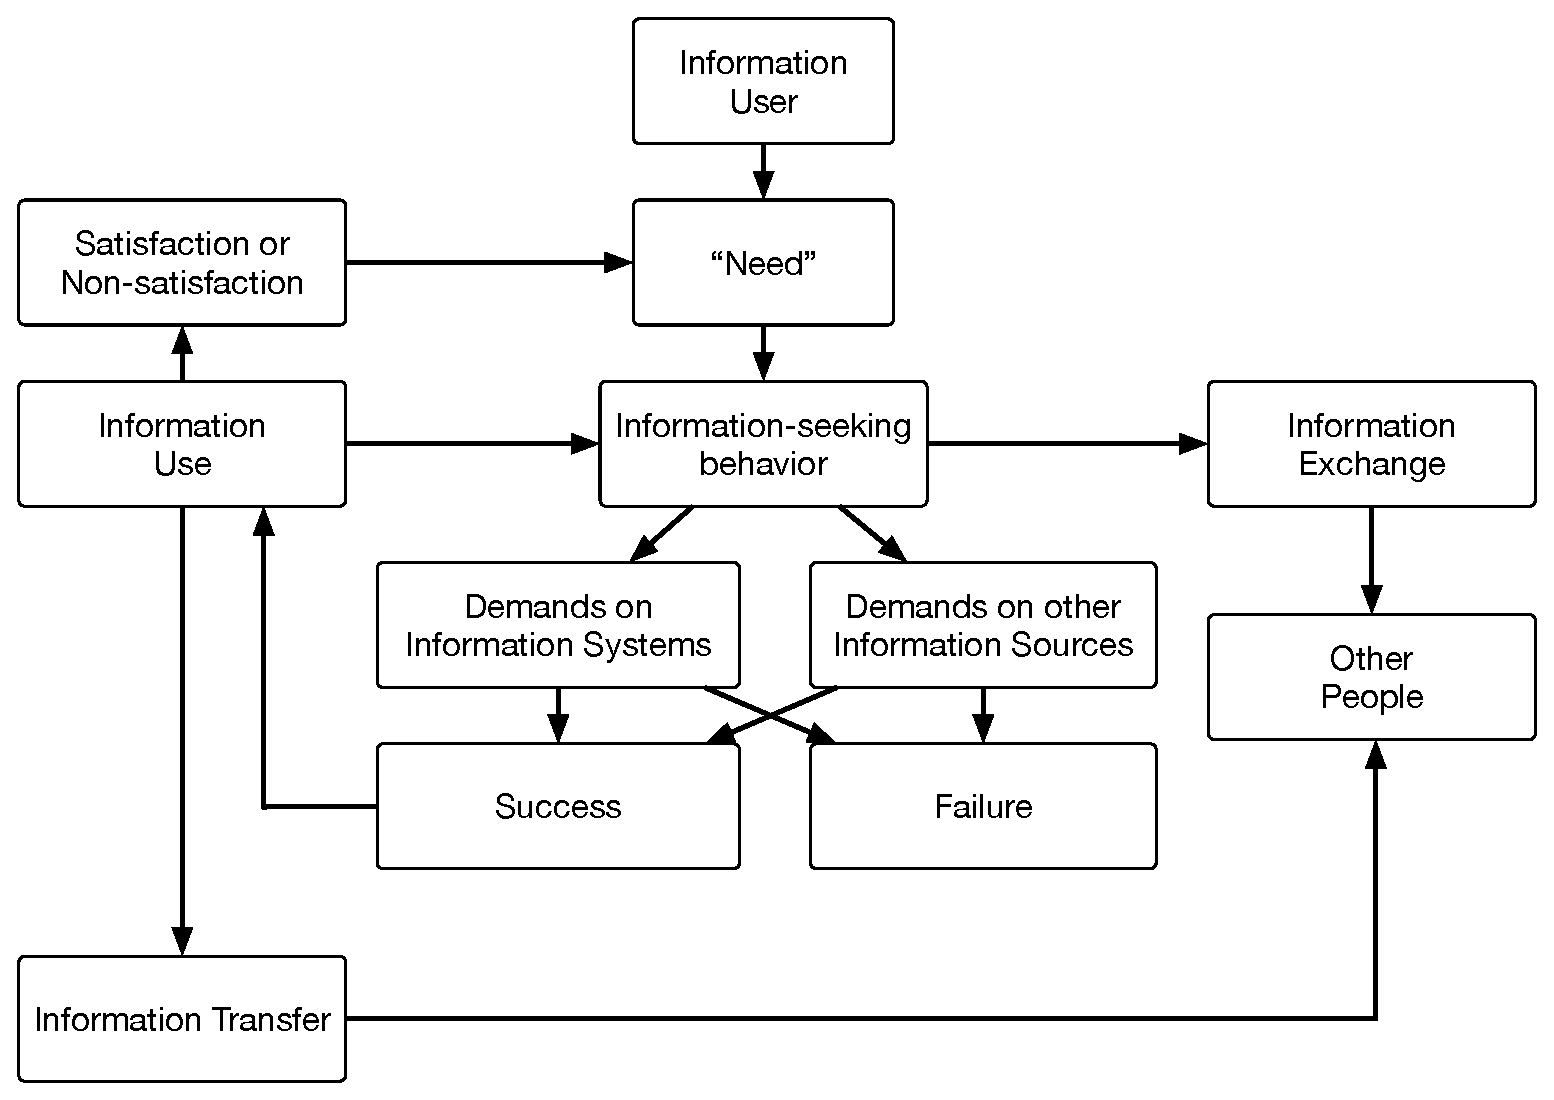
\includegraphics[width=0.7\textwidth]{figures/wilson-info-behavior}
    \caption{Wilson's information seeking behavior model \cite{wilson1981user}}
    \label{fig:wilson-info-seek}
\end{figure}

Wilson's model has been envolved many years since its origin, and it was revised 
and adapted to our digital world since the digital systems learns user preferences and 
changes \cite{giannini1998receiving} the way we receiving information.

David Ellis described a detailed group of activities for information seeking behavior \cite{ellis1989behavioural},
and then applied in physical and social science \cite{ellis1993comparison} and industrial
environment \cite{ellis1997modelling}.
In addition, his analysis was
based on grounded theory approach \cite{aceto1994grounded} and semi-structured interviews. 

Afterwards, Choo et al. adapts Ellis' Model and discussed \cite{choo1999information}
the information seeking behavior on the web through different activities rather 
than a single process, the applied activities are:
starting, chaining, browsing, differentiating, monitoring, and extracting.

``\emph{Starting}'' on the web indicates that a user identifies websites or pages
that containing the information of interests.
``\emph{Chaining}'' indicates that a user follows on starting page to other related pages.
``\emph{Browsing}'' then represents the activity that a user only skimming on the web
and quickly viewing the top-level informations. The ``\emph{differentiating}'' 
describes that a user on the web is selecting useful pages and choosing differentiated.
``\emph{Monitoring}'' activity is used for receiving updates on the sites, or revisit
the previously visited pages. Finally ``\emph{extracting}'' is the activity that a user
systematically extracts informations from a interested page or website.

By applying these activities, Choo et al concludes general user behaviors on the web are
undirected viewing, conditioned viewing, informal search and formal search.
Johnson further describes \cite{johnson2017patterns} seven more detailed behaviors 
patterns on the web, but did not given a working study that verify or prove their formation.

Although Wilson's model and Ellis' model are revised in recent works, however these improvements
are more generic and too complexy for describing user information behavior on the web.
Therefore, in this thesis, we only uses the an antecessor of Wilson's framework \cite{wilson1997information} and 
Ellis' model \cite{ellis1997modelling} to formalize and justify our lab study experiment later in Chapter \ref{ch:exp}, 
as a fundation of our work.

% \subsection{Theory of Sequence to Sequence Learning}

\cleardoublepage
\section{Experiment Design}

TODO

% - 介绍实验的具体细节,包括所有的实验任务
% - 为搜集任务的设计进行辩护,为什么任务是合理的,clickstream 和 searchstream 之间有什么区别
% - 在这里陈述搜集到的实验结果,包括 subjects 的总体数据

\cleardoublepage
\section{Model Design}

% - 阐述基于 RNN 的点击流模型,介绍如何通过这个模型对点击流进行预测,这个预测结果包括后续整个点击流的预测,
% - 模型需要能够对整条点击流进行一个评估,这个评估包含了

\cleardoublepage
\section{Implementation}

\subsection{Client-side architecture}

\subsubsection{Browser Market Share}

\subsubsection{Architecture: Chrome as Example}

\subsection{Server-side architecture}

% 讨论软件设计的客户端和服务端架构,讨论模型的部署相关的细节

\subsubsection{Model Evolution Automation Architecture}

\subsection{Communication Protocol}

\cleardoublepage
\section{Analysis}

% 分析实验结果,对比的实验结果包括:

%  任务本身的分析,对任务的难度进行讨论

\cleardoublepage
\section{Applications}

% - 针对分析得出的结果,讨论开发的插件、插件的实现架构
% - 讨论针对

\subsection{Client Side Browser Plugin}

\subsection{Standard Browser Web APIs}

\subsubsection{}

\cleardoublepage
\section{Conclusions}
\label{ch:final}

\subsection{Summary}

% 1. what has been done

This thesis proposed an action path model that describes client-side user clickstream.
To justify our model, we designed nine browsing tasks for three qualitatively
discussed browsing behavior based on the theory of information behavior, then 
held a user study for these tasks that simulates the behaviors. 
Afterwards, we applied the collected data from user study to our action path model and
analysed the model performance to these data with comparison to traditional machine 
learning approach.
Subsequently, we also visualized these data and closely discovered the common, 
individual and intersection patterns among client-side clickstream.
As an application show case, we illustrated a browser plugin that monitors client-side 
user clickstream to predict future movements of web browsing and discussed the benifits of this plugin.
Futhermore, we presented a generic architecture communication flow and architecture of the plugin, 
as well as the possibilities of standardize the plugin feature as browser Web APIs to other developers.

% 2. what are the findings

Our finding indicates the completion difficulty in different type of tasks are significant different,
especially the difficulty of fuzzy task is significant difficult than goal-oriented task,
and the goal-oriented task is also significant difficult than exploring task.
For completion efficiency, length of client-side clickstream and total duration of the clickstream

% 3. emphasize the importance >> place to large context
Our findings are generic and subservience. The model can not only be use on desktop but
also can be implemented in a mobilephone, or even a outside the context of web browsing. 
Similar to other user behavior data, client-side user clickstream or user actions 
directly indicates movements of a user and how they making decisions. Understanding, 
interpreting and predicting these data not only improves the user experience when doing
web browsing, but also useful to help users reducing useless browsing, better controls 
and manages their time. Moreover, by standardize the data processing process can formalize
the feature to developers, and then help them using the behavior predictions to
improve their product user experience.

% 4. summarize / conclude
Traditional server collected clickstream data has been proved its high value in many fields. With our work we exposit the value one-step forward, and contributes to models and approaches that hope to bring ponderable research to the community.


\cleardoublepage
\part*{Appendix}
\appendix
\addcontentsline{toc}{part}{Appendix}
% No headline on top of each page
\fancyhead[LE,RO,LO,RE]{}

All resources relates to the thesis are open source, they can be found publicly in:

\begin{itemize}
    \item Thesis homepage: \url{https://changkun.us/master-thesis-hci/};
    \item GitHub repostory: \url{https://github.com/changkun/MasterThesisHCI/}.
\end{itemize}

All related text, picture and video content are licensed under a Creative Commons Attribution-NonCommercial-ShareAlike 4.0 International License\footnote{\url{http://creativecommons.org/licenses/by-nc-sa/4.0/}}.
The other parts of the thesis (such as program source code) are licensed under a MIT Public License\footnote{\url{https://github.com/changkun/MasterThesisHCI/blob/master/LICENSE}}.

\section{Content of enclosed USB}
\label{appendix:a}

\begin{enumerate}
    \item $/documents/$ - TODO
\end{enumerate}

\part*{Bibliography}

\addcontentsline{toc}{part}{Bibliography}
\nocite{*}
\bibliographystyle{plain}
\bibliography{literature/list}
\end{document}